\clearpage
\phantomsection% 
\addcontentsline{toc}{chapter}{Lembar Pengesahan}


% \begin{center}

% 	\large \bfseries \MakeUppercase{Lembar Pengesahan}
    
%     \normalsize \normalfont \onehalfspacing \justify{
%     Tugas Akhir Sarjana dengan judul Tugas Akhir Sarjana dengan judul "IDENTIFIKASI PENYAKIT PADA DAUN BIBIT KELAPA SAWIT DENGAN PENDEKATAN NAÏVE BAYES MENGGUNAKAN OPTIMASI GENETIC ALGORITHM DAN PARTICLE SWARM OPTIMIZATION (Studi Kasus: PT Perkebunan Nusantara IV Regional 7 Kebun Bekri)"  adalah benar dibuat oleh saya sendiri dan belum pernah dibuat dan diserahkan sebelumnya, baik sebagian ataupun seluruhnya, baik oleh saya ataupun orang lain, baik di Institut Teknologi Sumatera maupun di institusi pendidikan lainnya.}

% 	% Informasi Mahasiswa
% 	\setlength{\tabcolsep}{0pt}
% 	\begin{tabular}{p{0.7\textwidth} p{0.3\textwidth}}
% 		Lampung Selatan, 21-05-2025 & %
% 		\multirow{6}{*}{
% 			% Kotak pasfoto 3x4
% 			\phantom{---} % Amazing hack biar kotaknya ke kanan (RDB)
% 			\begin{tikzpicture}
% 				\draw rectangle (3cm,4cm) node[pos=0.5] {Foto 3x4};
% 			\end{tikzpicture}
% 		}\\
% 		Penulis, \\
% 		& \\
% 		& \\
% 		& \\
% 		& \\
% 		\theauthor\\
% 		NIM \printnim
% 	\end{tabular}

% 	% Informasi Dosen
% 	\centering Diperiksa dan disetujui oleh,
% 	\justify
%     \setlength{\tabcolsep}{0pt}
%     \begin{tabular}{ m{0.5cm}  m{0.7\textwidth} >{\centering\arraybackslash}m{0.3\textwidth}}
%         \multicolumn{2}{c}{Pembimbing} & \multicolumn{1}{c}{Tanda Tangan} \\
% 		1. & \printnamadosbinga & \\
% 		 & \printnipdosbinga & ......................\\
% 		% 2. & \printnamadosbingb & \\
% 		%  & \printnipdosbingb & ......................\\
% 		& \\[0.25cm]
% 		%  & \\
% 		\multicolumn{2}{c}{Penguji} & \multicolumn{1}{c}{Tanda Tangan} \\
% 		1. & \printnamapengujia & \\
% 		& \printnippengujia & ......................\\
% 		2. & \printnamapengujib & \\
% 		& \printnippengujib & ......................\\
%     \end{tabular}
% %	\vfill

% 	\begin{center}
% 		\fontsize{10pt}{12pt}
% 		Disahkan oleh,\\
% 		Koordinator Program Studi Teknik Informatika\\
% 		Fakultas Teknologi Industri\\
% 		Institut Teknologi Sumatera
% 		\vspace{2cm}\\
% 		Andika Setiawan, S.Kom., M.Cs. \\ % TODO: make automatic
% 		NIP 19911127 2022 03 1 007 \\
% 	\end{center}
% 	\vfill

% \end{center}
% \clearpage


\clearpage
\pagestyle{fancy}
\fancyhf{}
\fancyhead[R]{\thepage}
\phantomsection% 
\addcontentsline{toc}{chapter}{LEMBAR PENGESAHAN}

\begin{center}

	\large \bfseries \MakeUppercase{Lembar Pengesahan}
    
    \small \normalfont \singlespacing \justify{
    Tugas Akhir Sarjana dengan judul 
	"IDENTIFIKASI PENYAKIT PADA DAUN BIBIT KELAPA SAWIT DENGAN PENDEKATAN NAÏVE BAYES MENGGUNAKAN OPTIMASI GENETIC ALGORITHM DAN PARTICLE SWARM OPTIMIZATION (Studi Kasus: PT Perkebunan Nusantara IV Regional 7 Kebun Bekri)" adalah benar dibuat oleh saya sendiri dan belum pernah dibuat dan diserahkan sebelumnya, baik sebagian ataupun seluruhnya, baik oleh saya ataupun orang lain, baik di Institut Teknologi Sumatera maupun di institusi pendidikan lainnya.}
	\vspace{0.1cm}
    %Dengan ini saya menyatakan bahwa Tugas Akhir Sarjana berjudul "{\thetitle}" adalah karya orisinal saya. Tugas akhir ini belum pernah diserahkan atau diterbitkan sebelumnya, baik sebagian maupun seluruhnya, oleh saya atau pihak lain, di Institut Teknologi Sumatera maupun institusi pendidikan lainnya.
    %Saya menyatakan bahwa Tugas Akhir berjudul "{\thetitle}" merupakan hasil karya saya sendiri dan belum pernah diajukan, baik sebagian maupun seluruhnya, di Institut Teknologi Sumatera atau institusi pendidikan lain oleh saya maupun pihak lain.

	% Informasi Mahasiswa
	\setlength{\tabcolsep}{0pt}
	\begin{tabular}{p{0.59\textwidth} p{0.3\textwidth}}
        \vspace{0.1cm}
		Lampung Selatan, 21 Mei 2025 & %
		\multirow{6}{*}{
			% Kotak pasfoto 3x4
			\phantom{---} % Amazing hack biar kotaknya ke kanan (RDB)
			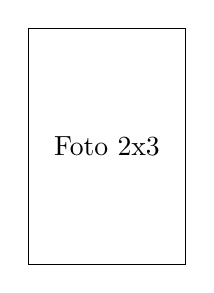
\begin{tikzpicture}
				\draw rectangle (2cm,3cm) node[pos=0.5] {Foto 2x3};
			\end{tikzpicture}
		}\\
		Penulis, \\
		& \\
		& \\
		%& \\
		\theauthor\\
		NIM \printnim
	\end{tabular}
	% Informasi Dosen
	\vspace{0.3cm}
        \begin{center}
        Diperiksa dan disetujui oleh,
        \end{center}
        \vspace{0.3cm}

	\justify
    \setlength{\tabcolsep}{0pt}
    \begin{tabular}{ m{0.5cm}  m{0.7\textwidth} >{\centering\arraybackslash}m{0.3\textwidth}}
        \multicolumn{2}{c}{\hspace*{-50pt}Pembimbing} & \multicolumn{1}{c}{Tanda Tangan} \\[2pt]
		1. & \printnamadosbinga & \\
		 & \printnipdosbinga & ............. \\[4pt]
		 %& \\
		\multicolumn{2}{c}{\hspace*{-70pt}Penguji} & \multicolumn{1}{c}{Tanda Tangan} \\[2pt]
		1. & \printnamapengujia & \\
		& \printnippengujia & ............. \\[4pt]
            %& \\
		2. & \printnamapengujib & \\
		& \printnippengujib & ............. \\
    \end{tabular}
%	\vfill

	\begin{center}
		\fontsize{10pt}{10pt}
        \vspace{0.35cm}
		Disahkan oleh,\\
		Koordinator Program Studi Teknik Informatika\\
		Fakultas Teknologi Industri\\
		Institut Teknologi Sumatera
		\vspace{1cm}\\
		Andika Setiawan, S.Kom., M.Cs. \\ % TODO: make automatic
		NIP 19911127 2022 03 1 007 \\
	\end{center}
	\vfill

\end{center}
\clearpage